\chapter{Anwendungen von Docker}
\label{cha:anwendungen_von_docker}
Das Hauptanwendungsgebiet von Docker befindet sich im Bereich des Cloud Computing. Hier kann Docker vor allem in den Architekturvarianten Platform as a Service und Software as a Service punkten. Darüber hinaus kann Docker noch in zahlreichen weiteren Bereichen sinnvoll zum einsatz gebracht werden. Einen besonders wichtigen Bereich bildet hier die Automatisierung von Tests in der Softwareentwicklung (siehe Abb \ref{fig:anwendungsfaelle}).
Im Folgenden wird die Software Docker kurz beleuchtet um die wichtigsten Eigenschaften noch einmal hervorzuheben. Es wird allerdings davon ausgegangen, dass Docker dem Leser bereits ein Begriff ist. Docker wird daher nicht mehr im Detail beschrieben. Im weiteren wird dann auf die genannten Anwendungsfälle näher eingegangen.
\begin{figure}[htbp]
  \centering  
  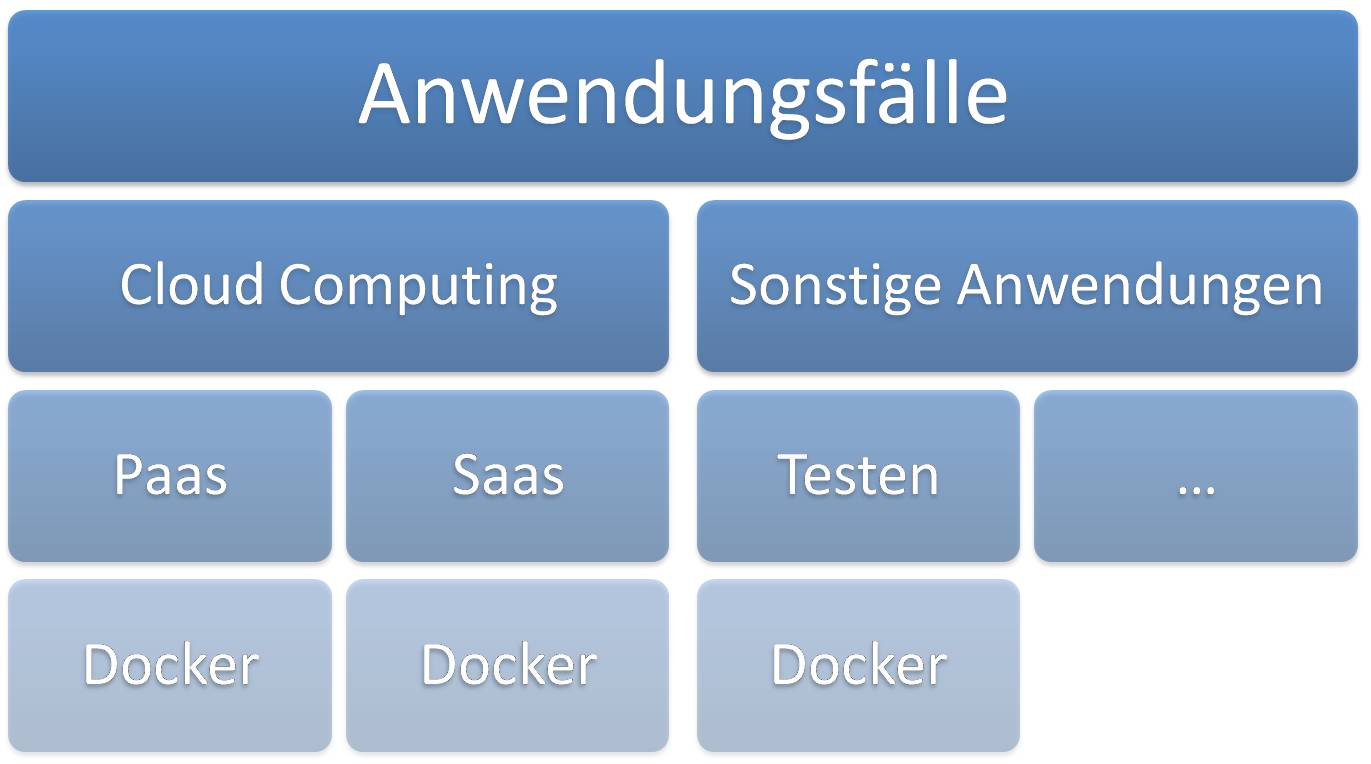
\includegraphics[scale=0.7]{img/anwaendungsfaelle.jpg}\\
  \caption{Die behandelten Anwendungsfälle im Überblick}
  \label{fig:anwendungsfaelle}
\end{figure}

\section{Docker}
\label{sec:docker}
Docker ist eine Software, die es ermöglicht Anwendungen zusammen mit ihren Abhängigkeiten in einen isolierten Container zu verpacken. Docker bedient sich dabei der Linux eigenen LXC Conntainer Technologie und erweitert diese um eine simple Benutzer API (Application Pro-
gramming Interface) zum erzeugen, verwalten und für die Interaktion mit diesen Containern.
Die Eigenschaften von Docker können dabei wie folgt zusammengefasst werden: \cite{abel_docker:_2013}
\begin{itemize}
 
      \item \textbf{Dateisystem Isolation} \\
Jeder Prozess läuft in einem seperaten root-Dateisystem
      \item \textbf{Resourcen Isolation} \\
Systemressourcen wie CPU und Speicher können für jeden Container einzeln geregelt werden.
      \item \textbf{Netzwerk Isolation} \\
Jeder Prozess-Container läuft in seinem eigenen Netzwek-Namensraum mit einer separaten, 			virtuellen Netzwekschnittstelle und IP-Adresse.
      \item \textbf{Copy-On-Write} \\
Änderungen am Dateisystem eines Containers werden in eine neue Schicht gespeichert und nicht in das originale Abbild übernommen. Dies erlaubt ein schnelles Anlegen neuer Container und spart sowohl Arbeits- als auch Festplattenspeicher.
      \item \textbf{Protokollierung} \\
Die Standard-Datenströme (stdout/stderr/stdin) jedes Containers werden protokolliert, um in Echtzeit oder als Stapel bearbeitet zu werden.
	  \item \textbf{Änderungsverwaltung} \\
Änderungen an Dateien in einem Container können zu einem neuen Abbild zusammengesetzt werden. Dieses kann als Grundlage für neue Container dienen.
	  \item \textbf{Interaktive Shell} \\
Docker kann ein Pseudo-Terminal anlegen und mit den Standard-Datenströmen verbinden, um eine interaktive Verbindung mit einem Container zu ermöglichen.
\end{itemize}
Docker wird seit März 2013 von der Firma dotCloud (seit Oktober 2013 Docker
Inc.) unter der Apache Lizenz 2.0 veröffentlicht.\cite{github_dotcloud/docker_2013}
Im folgenden sollen mögliche Anwendungsfälle von Docker näher beleuchtet werden.
\section{Paas}
\label{sec:paas}
Die Firma dotCloud ist ein Platform as a Service-Provider. Als Erfinder und treibende Kraft hinter dem Docker-Projekt ist es also nicht verwunderlich, dass das Hauptanwendungsfeld von Docker im Bereich von Platform as a Service liegt.
Docker ist eigentlich eine Neuentwicklung eines Teils des Systems, welches sich dotCloud über die Jahre als 
Platform as a Service-Provider angeeignet hat. DotCloud verfolgt mit Docker das Konzept, einen Grundstein vorzugeben um den eine Platform as a Service-Infrastruktur aufgebaut werden kann.\cite[Zeit 18:24]{hykes_introduction_2013}

Um zu verstehen welche Vorteile Docker als Basis einer Platform as a Service-Infrastruktur bieten kann, müssen zunächst die Probleme betrachtet werden, welchen sich ein Platform as a Service-Provider in der heutigen Zeit ausgesetzt sieht.

\subsection{Probleme von Paas}
\label{sec:probleme_von_paas}

Das Ausliefern von Code bzw. Software ist in der heutigen Zeit ein kompliziertes Unterfangen geworden. Aber wieso ist das so? Solomon Hykes, der Gründer von dotCloud, sieht den Grund hierfür in den immer komplexeren Hardware- und Software-Stack mit denen wir uns in der heutigen Zeit konfrontiert sehen. \cite{hykes_introduction_2013} 
Vor nicht allzu langer Zeit bestand ein typischer Hardware- und Software-Stacks noch aus einem simplen Server, dekoriert mit einer LAMP (Linux Apache MySQL PHP) Installation.
In den letzten Jahren haben sich jedoch sowohl der Hardware- als auch der Software-Stack deutlich verkompliziert. (siehe Abb \ref{fig:hardware_software_stack}) 
\begin{figure}[htbp]
  \centering  
  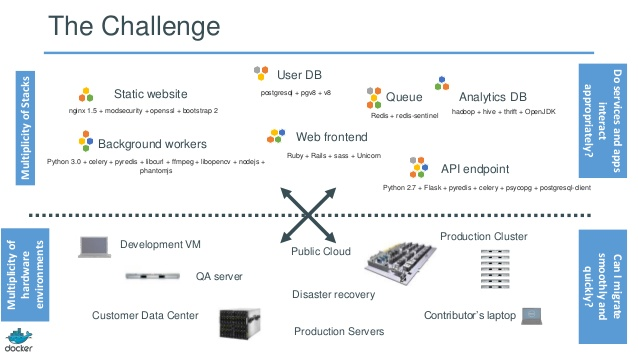
\includegraphics[scale=0.5]{img/hardware_software_stack.jpg}\\
  \footnotesize\sffamily\textbf{Quelle:} \cite{hykes_docker_2013}
  \caption{Unterschiedliche Hardware- und Software-Stacks}
  \label{fig:hardware_software_stack}
\end{figure}
Der Software-Stack reduziert sich nicht mehr auf eine simple Anwendung. Im Rahmen von Serviceorientierten Architekturen kommunizieren vielmehr viele verschiedene Stacks untereinander. Die einzelnen Stacks können sich dabei enorm unterscheiden was zum Beispiel die Programmiersprache oder die verwendeten Framewoks betrifft.
Plötzlich muss man nicht mehr nur einen einzelnen Software Stack isoliert betrachten sondern zusätzlich eine ganze Reihe von Services und deren Kommunikation untereinander.
Diese Vielzahl von Software-Stacks muss darüber hinaus auf einer immer komplexer werdenden Hardware-Infrastruktur betrieben werden. Entwickelte Software muss nicht mehr nur auf einem einzigen Server laufen sondern auf einer Vielzahl von unterschiedlicher Hardware wie z.b. Test-Server, Entwicklungs-Pc, Laptop, Produktiv-Server etc.
Wir betreiben also einen immer komplexeren Software-Stack auf einer immer komplizierteren Hardware-Infrastruktur. Dabei muss sichergestellt sein, dass jeder einzelne Software-Stack auf jeder Infrastrukturkomponente betrieben werden kann und dabei immer das selbe Verhalten zeigt.
Das Ergebnis ist eine Matrix von Abhängigkeiten zwischen Software-Stacks und Hardware die mit jeder neuen Komponente rasant an Komplexität gewinnt.
Solomon Hykes bezeichnet diese Matrix als \glqq Matrix From Hell\grqq \cite[Zeit 4:30]{hykes_introduction_2013}(siehe Abb \ref{fig:matrix_from_hell}) 

\begin{figure}[htbp]
  \centering  
  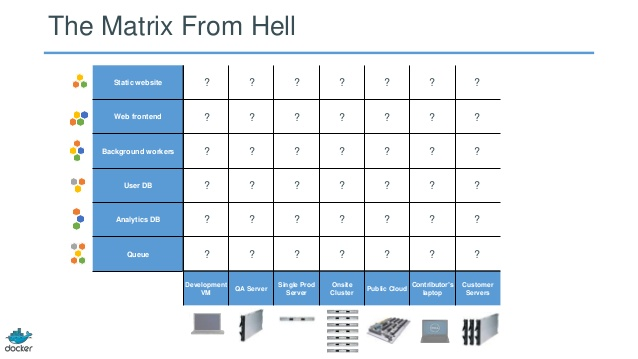
\includegraphics[scale=0.7]{img/matrix_from_hell.jpg}\\
  \footnotesize\sffamily\textbf{Quelle:} \cite{hykes_docker_2013}
  \caption{Matrix From Hell}
  \label{fig:matrix_from_hell}
\end{figure}

\subsection{Analogie mit der Frachtschifffahrt}
\label{sec:analogie_mit_der_frachtschifffahrt}
In der frühen Frachtschifffahrt sah man sich mit einem ähnlichen Problem konfrontiert und fand eine Lösung. Frachtschiffe müssen eine Vielzahl von Waren von einem Punkt A zu einem Punkt B transportieren. Analog zu unseren Software-Stacks können die Ware dabei völlig unterschiedliche Formen annehmen. Das Reicht beispielsweise von Autos über Elektronikgeräte bis hin zu kleinen Kaffeebohnen. All diese unterschiedlichen Gegenstände müssen auf ihrer Reise eine Vielzahl von Stationen analog zu unserer Hardware durchlaufen. (siehe Abb \ref{fig:waren_stationen}) 
\begin{figure}[htbp]
  \centering  
  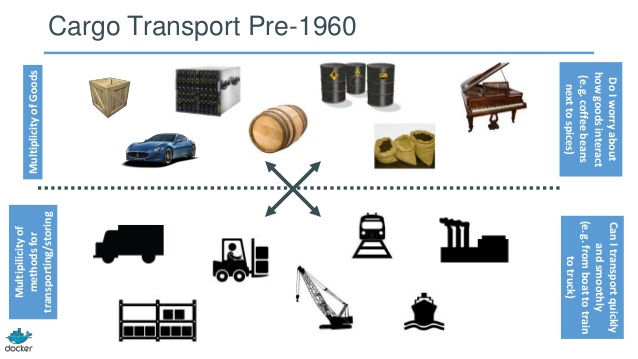
\includegraphics[scale=0.7]{img/waren_stationen.jpg}\\
  \footnotesize\sffamily\textbf{Quelle:} \cite{hykes_docker_2013}
  \caption{Waren und ihre Stationen in der Frachtschifffahrt}
  \label{fig:waren_stationen}
\end{figure}

Prinzipiell müssen dabei alle Waren gleich behandelt werden. Auf Grund ihrer unterschiedlichen Beschaffenheiten ist dies jedoch nicht ohne weiteres möglich. Ein Auto muss zum Beispiel anders verladen werden als ein Sack Kaffeebohnen.
Kombiniert man wieder alle möglichen Waren mit allen Stationen die sie auf ihrer Reise durchlaufen müssen, ergibt sich ein ähnliches Bild wie in der \glqq Matrix From Hell\grqq Abb \ref{fig:matrix_from_hell}. (siehe Abb \ref{fig:waren_matrix_from_hell_ii}) 
\begin{figure}[htbp]
  \centering  
  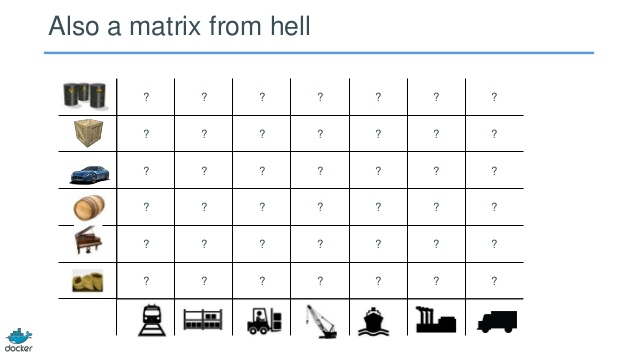
\includegraphics[scale=0.7]{img/waren_matrix_from_hell.jpg}\\
  \footnotesize\sffamily\textbf{Quelle:} \cite{hykes_docker_2013}
  \caption{Matrix From Hell II}
  \label{fig:waren_matrix_from_hell_ii}
\end{figure}

Die Lösung für dieses Problem ist der sogenannte Schiffscontainer. Alle Waren wenden bevor sie verschifft werden in einen einheitlichen, genormten Container verpackt. Die gesamte Infrastruktur kann sich somit auf ein einheitliches Format für zu verschiffende Waren standardisieren. Man schafft damit eine klare Trennung der Aufgabenbereich von Versender und Frachtschifffahrt. Die Infrastruktur muss sich nicht mehr darum kümmern wie einzelne Waren zu behandeln sind, sie verschifft nur noch Container und behandelt diese immer gleich. Der Versender der Waren hat sich hingegen nur noch darum zu kümmern, seine Güter in den Container zu verpacken. (siehe Abb \ref{fig:shipping_container})
\begin{figure}[htbp]
  \centering  
  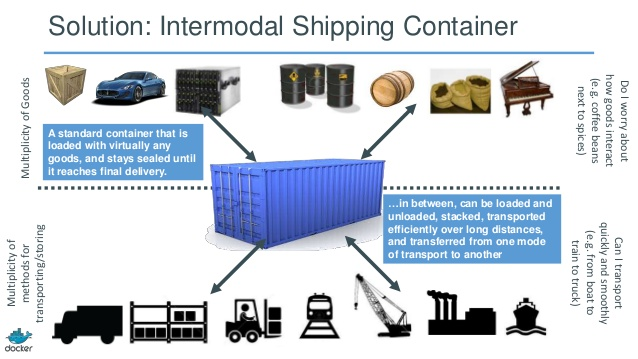
\includegraphics[scale=0.7]{img/shipping_container.jpg}\\
  \footnotesize\sffamily\textbf{Quelle:} \cite{hykes_docker_2013}
  \caption{Frachtcontainer}
  \label{fig:shipping_container}
\end{figure}

\subsection{Docker und Paas}
\label{sec:docker_und_paas}
Docker versucht genau dieses Konzept auf die Softwarewelt zu übertragen. 
Software wird nicht mehr einfach nur lose ausgeliefert sondern in einen standardisierten Container gepackt. Der Entwickler kümmert sich dabei um das Innenleben des Containers. Die restliche Infrastruktur kümmert sich nur noch darum, wie sie mit einem Container umzugehen hat. Für beide Welten definiert Docker über ein klar spezifiziertes Interface die Spielregeln. (siehe Abb \ref{fig:container_fuer_code})
\begin{figure}[htbp]
  \centering  
  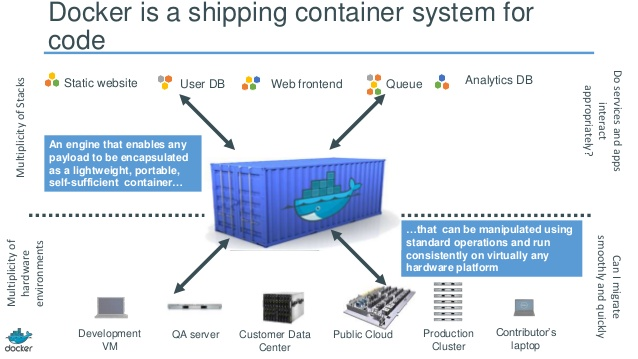
\includegraphics[scale=0.7]{img/hardware_software_container.jpg}\\
  \footnotesize\sffamily\textbf{Quelle:} \cite{hykes_docker_2013}
  \caption{Docker-Container für Code}
  \label{fig:container_fuer_code}
\end{figure}

Mit Hilfe von Docker ist es somit möglich die zuvor beschiedene \glqq Matrix From Hell\grqq Abb \ref{fig:matrix_from_hell} aufzulösen. Wird die Software in einer standardisierten weise gekapselt, kann sichergestellt werden, dass die Abhängigkeiten zwischen den einzelnen Software-Stacks nicht verändert werden und immer gleich funktionieren. Sie sind sozusagen bereits vor der Auslieferung fest im Container verankert. Der Infrastruktur muss nur noch beigebracht werden mit einem Container umzugehen, nicht mehr aber mit vielen verschiedenen Software-Stacks. Das stellt jedoch kein größeres Problem dar, da über das standardisierte Interface die Schnittstellen bereits für alle Anwendungen gleich vorgegeben sind. (siehe Abb \ref{fig:aufgeloesste_matrix_from_hell})
\begin{figure}[htbp]
  \centering  
  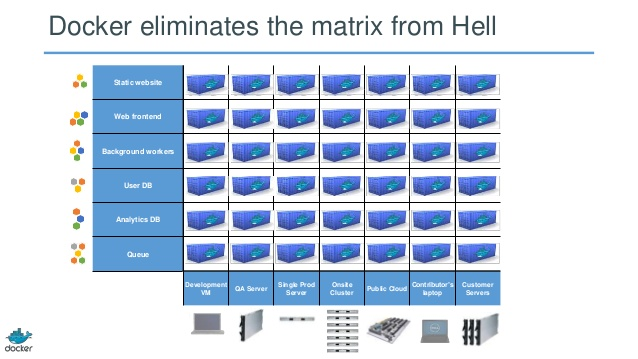
\includegraphics[scale=0.7]{img/aufgeloesste_matrix_from_hell.jpg}\\
  \footnotesize\sffamily\textbf{Quelle:} \cite{hykes_docker_2013}
  \caption{Aufgelößte Matrix From Hell}
  \label{fig:aufgeloesste_matrix_from_hell}
\end{figure}

Mit Hilfe von Docker ist es damit möglich einen großen Interessenskonflikt zwischen Platform as a Service-Provider und Platform as a Service-Nutzer zu beseitigen.
Der Nutzer möchte in der Regel eine möglichst große Freiheit. Er möchte selbst bestimmen wie die Abhängigkeiten seiner Software sind, welche Frameworks er verwendet oder in welcher Programmiersprache er seine Software implementiert. Er möchte sich nicht vorschreiben lassen unter welchen Rahmenbedingungen er seine Software umsetzt. Der Platform as a Service-Provider hingegen möchte möglichst kosteneffizient arbeiten und daher einen möglichst geringen Verwaltungsaufwand betreiben. Das bedeutet für ihn möglichst genaue Parameter festzulegen. Für ihn gibt es optimaler weise eine Programmiersprache, ein Framework, so dass am Ende alle auf der Plattform erzeugten Anwendungen gleich zu handhaben sind. Dieser Interessenskonflikt muss zwangsläufig in irgend einer Art von Kompromiss aufgelöst werden.
Eine für beide optimale Lösung wäre nach Solomon Hykes \cite[Zeit 13:50]{hykes_introduction_2013} die Verwendung von virtuellen Maschinen. Der Nutzer hätte die maximal mögliche Freiheit beim Packen seiner Anwendung. Der Provider müsste sich nur auf das betreiben von virtuellen Maschinen spezialisieren. Dieses Konzept ist jedoch nicht praktikabel. Der Overhead an Daten wäre hierbei einfach viel zu groß. Im Grunde würde man für jede Anwendung immer einen komplette Rechner ausliefern. Darüber hinaus müsste man einige Einbußen im Bereich der Performance hinnehmen.
\glqq Virtualisierung fügt eine weitere Abstraktionsschicht zu einem System hinzu (siehe Abb \ref{fig:abstraction_container_hyper} Hypervisor-based Virtualization), was unweigerlich einen Geschwindigkeitsverlust gegenüber des direkten Betriebs einer Anwendung bedeutet. Zu unterscheiden sind Zwei Arten: die Verzögerung beim Starten der Anwendung und das langsamere Ausführen verschiedener Operationen während des Betriebs.\grqq \cite[Seite 4]{schroder_container-virtualisierung_2014}
Für einen Platform as a Service-Anbieter kann hier vor allem die langsamere Ausführung von Operationen durchaus zum Problem werden.
Mit Hilfe von Docker ist es möglich diese Lücke zu schließen. Durch eine dünnere Abstraktions-Schichten ist die Geschwindigkeit der virtualisierten Programme in einem Container fast identisch mit der von direkt auf dem System laufenden Programmen (siehe Abb \ref{fig:abstraction_container_hyper} Vontainer-based Virtualization).\cite{schroder_container-virtualisierung_2014}
\begin{figure}[htbp]
  \centering  
  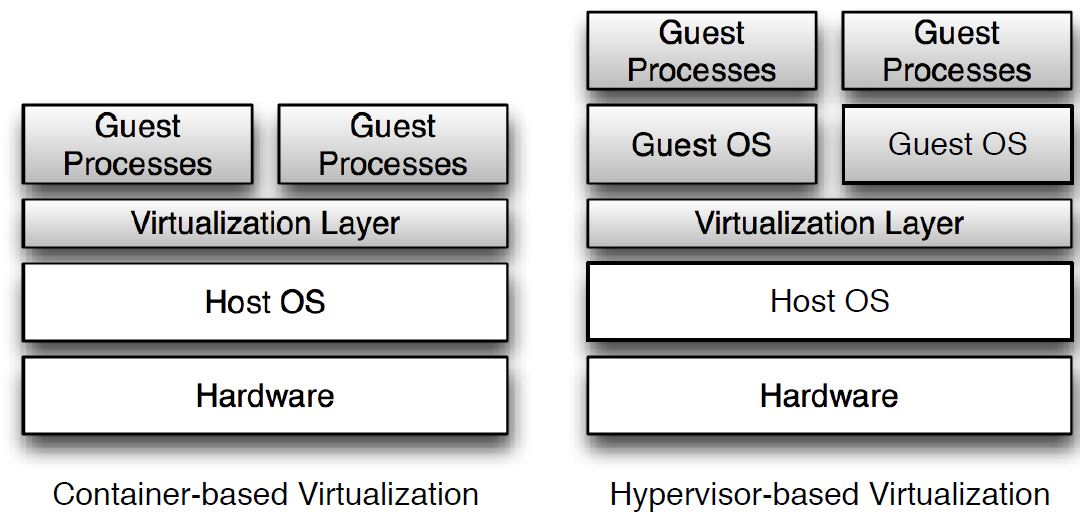
\includegraphics[scale=0.5]{img/abstractionContainerHyper.JPG}\\
  \footnotesize\sffamily\textbf{Quelle:} \cite{miguel_g._xavier_performance_????}
  \caption{Vergleich von Container- und Hypervisorbasierter Virtualisierung }
  \label{fig:abstraction_container_hyper}
\end{figure}
Auch der Overhead an Daten beim ausliefern einer in einen Container gepackten Anwendung ist so gering, dass er kein Argument mehr darstellt diese nicht zu verwenden.
Docker eliminiert also große Probleme welche die Verwendung von virtuellen Maschinen mit sich bringen würde, hat dabei aber den selben großen Vorteil.
Der Entwickler ist innerhalb des Containers frei. Er kann alle Parameter selbst so festlegen, dass sichergestellt ist, dass sich die Anwendung die er lokal getestet hat auch auf der Infrastruktur des Platform as a Service-Providers noch genauso verhalten wird. 
Docker bildet somit die optimale Basis um darum eine effiziente Platform as a Service-Infrastruktur aufzubauen. 

\section{Saas}
\label{sec:saas}
Die Grenzen zwischen Platform as a Service und Software as a Service sind fliesend.
Verwendet man Docker wie bereits im Abschnitt \ref{sec:docker_und_paas} gezeigt als Kern einer Platform as a Service-Umgebung, um darauf wiederum Software bereitzustellen, verwendet man Docker im Grunde bereits zum betreiben von Software as a Service.

\subsection{Docker und Saas}
\label{sec:docker_und_saas}
Docker kann darüber hinaus jedoch auch explizit zur Implementierung einer Software as a Service-Lösung verwendet werden. Jede Instanz der angebotenen Softwarelösung wird dabei in einen eigenen Container verpackt. Mit Hilfe eines sogenannten \grq Dockerfiles\grq\ kann das Innenleben eines Containers genau definiert werden. Ein Dockerfile enthält dazu eine Reihe von Dockerbefehlen die später sequentiell ausgeführt werden sollen. Compiliert man ein solches Dockerfile entsteht daraus ein Abbild des gewünschten Systems welches als \grq Dockerimage\grq\ bezeichnet wird.
Dieses Image kann nun verwendet werden um beliebig viele immer gleiche Instanzen in Form von Docker Containern zu erzeugen.
Hier wird deutlich wie Docker das Anbieten einer Software mittels Software as a Service unterstützen kann.
Die gewünschte Software muss nur einmal innerhalb eines Dockerimage definiert werden. Für jeden Benutzer der eine Instanz der Software as a Service-Lösung benötigt muss also nur noch ein eigener Container aus diesem Image erzeugt werden. Alles was man also neben einem funktionsfähigem Image noch benötigt um eine Software als Software as a Service mit Hilfe von Docker anzubieten ist eine Webanwendung die das erzeugen, verwalten und Bereitstellen der Container für die einzelnen Benutzer übernimmt.
Ein mögliches Anwendungsgebiet wäre dann zum Beispiel, Nutzern auf einfache und unkomplizierte Art und Weise Testinstanzen eine neuen Software bereitzustellen und somit das eigene Produkt zu vermarkten.
Juien Barbier hat eine Beispielanwendung erstellt die zeigen soll, dass dieses Konzept auch in der Praxis umgesetzt werden kann.
In seinem Projekt \glqq Build Your Own SaaS with Docker\grqq \cite{barbier_build_2013} hat er eine einfache Webanwendung erstellt mit deren Hilfe Docker Container erzeugt und bereitgestellt werden können. Mit seiner Anwendung ist es möglich den Cache-Server \grq Memcached\grq\ als Software as a Service über das Internet anzubieten. Mit wenigen Maus-klicken können sich Benutzer eine eigene Memcached Instanz erzeugen und diesen über das Internet ansprechen.
Im Hintergrund wird dafür aus einem vordefinierten Image ein neuer Docker Container mit einer laufenden Memcached-Instanz erzeugt.
Paul Czarkowski hat in einer ähnlichen Anwendung mit dem selben Vorgehen einen  IRC Bouncer als Software as a Service erstellt. Dabei hat er gezeigt, dass selbst mit einem Server mit nur 512 mb Hauptspeicher das betreiben von einhundert gleichzeitigen Instanzen problemlos möglich ist. \cite{czarkowski_i_????}
Mit Hilfe von Docker kann man also auf recht simple Art und Weise eine Vielzahl von unterschiedlichen Anwendungen als Software as a Service zu betreiben.

\section{Automatisierung von Tests mit Docker}
\label{sec:automatisierung_von_tests_mit_docker}

Die bisher beschriebenen Anwendungsgebiete befinden sich alle im Bereichen die in Architekturvarianten der Cloud angesiedelt sind. Also einem Gebiet, für das Docker gedacht ist und entwickelt wurde. Neben diesen Anwendungsgebieten bieten sich aber noch zahlreiche weitere Bereiche in denen Docker sinnvoll eingesetzt werden kann.
Einer davon ist die Verwendung von Docker für die Automatisierung von Tests in der Softwareentwicklung.

Ein heute weitverbreitetes vorgehen zur Optimierung der Softwareentwicklung ist \grq Continuous Integration\grq . Unter \grq Continuous Integration\grq\ versteht man ein vorgehen in der Softwareentwicklung bei dem alle Mitglieder eines Teams ihre Änderungen am Code besonders häufig integrieren, also zusammenführen. Üblich sind hier durchaus mehrere Integrationen pro Tag. 
\glqq Im Team entwickelte Softwareprojekte sind mit wachsender Größe und Komplexität zunehmend schwieriger zu verwalten und zu bauen. Durch das ständige Zusammenspiel vieler Entwickler schleichen sich früher oder später zwangsläufig sogenannte Integrationsfehler ein, die sich, je nachdem wann sie bemerkt werden, nur schwer oder gar nicht mehr beseitigen lassen.\grqq \cite{feustel_continuous_????}
Dieser Entwicklung soll das Vorgehen von \grq Continuous Integration\grq\ entgegenwirken.
Jede Integration wird von einem automatisiertem \grq build\grq\ der Anwendung begleitet. Bei jedem \grq build\grq\ werden eine Reihe von automatisierten Tests durchgeführt. So können Integrationsfehler frühzeitig erkannt und behoben werden.

Hat das zu testende System viele Abhängigkeiten zu Fremdsystemen können diese Tests mitunter schnell recht komplex werden. Oftmals bekommt man diese Problematik noch über die Verwendung von Mockups in den Griff. Handelt es sich bei den auszuführenden Tests jedoch um Akzeptanztests die eine Bedienung der Anwendung über das Benutzerinterface simulieren sind schnell die Grenzen von klassischen Mockups erreicht.
In diesem Fall müssen wohl oder übel alle Abhängigkeiten der Anwendung auch tatsächlich vorhanden sein. Bei Anwendungen mit vielen Abhängigkeiten wird das schnell zum Problem.
Arbeitet man mit mehreren Systemumgebungen müssen alle Abhängigkeiten mehrfach bereitgestellt werden, was einen hohen Kostenaufwand bedeuten kann.
Benötigt eine Anwendung zum Beispiel im Hintergrund einen LDAP-Server für die Authentifizierung und das Projekt arbeitet mit einem Entwicklungs-, Test- und Produktions-System muss der selbe Server drei mal bereitgestellt werden.
Möchte man diese Akzeptanztests, wie es heute üblich ist, auch noch von jedem Entwicklungsrechner aus ausführen können, würde man streng genommen zusätzlich für jeden Entwickler eine eigenen Peripherie benötigen.
Von der Vielzahl der Instanzen der Abhängigkeiten einmal abgesehen, bekommt man mit diesem Vorgehen noch einen weiteren unschönen Effekt.
Man muss sich nicht mehr nur Gedanken über sein eigenes System machen, sondern ist immer angewiesen auf die Richtigkeit aller Abhängigkeiten.
Fällt zum Beispiel nur eine der Abhängigkeiten aus, ist sofort der gesamte Workflow der \grq Continuous Integration\grq\ gestört.
Änderungen die Abhängigkeiten des Systems betreffen müssen darüber hinaus an einer Vielzahl von stellen vorgenommen werden, was die Wartbarkeit zusätzlich erschwert.
Die Lösung für diese Probleme liegt in der Virtualisierung.
Um die starke Koppelung mit den Fremdsystemen bei der Ausführung von Tests aufzulösen und die Tests somit konstant und reproduzierbar zu machen, ist man dazu übergegangen die Abhängigkeiten in Form von virtuellen Maschinen bereitzustellen.
Benötigt ein Test also zum Beispiel die Präsenz eines LADP Servers, startet er sich diesen einfach für die benötigte Zeit als virtuelle Instanz mit den gewünschten Eigenschaften.
Werkzeuge wie Chef, Puppet und Vagrant machen es besonders einfach die Eigenschaften einer virtuellen Maschine im Vorhinein festzulegen und sie anschließend mit nur einem Befehl zu starten.
Auf leistungsstarken Systemen kommt man mit diesem vorgehen sehr gut zurande. Möchte man allerdings dem Wunsch der Entwickler nachkommen automatisierte System- und Akzeptanztests in einer produktionsnahen Umgebung vollständig lokal auf dem Entwicklungsrechner durchzuführen läuft man hier schnell in Performanceprobleme.
Wenn die Infrastruktur \glqq ausreichend produktionsähnlich, also komplex wird, mit verschiedenen interagierenden Anwendungsservern und Datenbanken auf verschiedenen Virtuellen Maschinen, dann reichen die Ressourcen eines Entwicklungsrechners zum Ausführen einer solchen Umgebung oft nicht aus. Das liegt mitunter daran, dass jede Virtuelle Maschine ein eigenes vollständiges Betriebssystem inklusive Kernel, Bibliotheken, Netzwerk-Stack usw. in den Arbeitsspeicher steckt.\grqq \cite{holbreich_von_2014}

Hier kann Docker eine ernstzunehmende Alternative für die bisherigen Tools darstellen. Ersetzt man die \grq schweren\grq\ virtuellen Maschinen durch leichtgewichtige Container ist es möglich, sehr viel komplexere Infrastrukturen auch mit minimalen Systemressourcen zu betreiben.
Aufgrund einer geringeren Abstraktionsschicht (siehe Abb \ref{fig:abstraction_container_hyper}) bieten die leichtgewichtigen Container einen signifikanten Performancegewinn gegenüber der klassischen Virtualisierung welcher es zusammen mit einem geringeren Arbeitsspeicherauslastung ermöglicht zahlreiche Container auch auf schwächeren Entwicklungsrechnern zu betreiben.
Xavier et al. \cite{miguel_g._xavier_performance_????} haben dazu einen Performancevergleich zwischen klassischer hypervisorbasierter Virtualisierung und Containerbasierter Virtualisierung angestellt.
In diesem Vergleich wurden gängige Container  wie Linux VServer, OpenVZ and Linux Containers (LXC) einem Vertreter der hypervisorbasierten Virtualisierung: Xen gegenübergestellt.
Docker benutzt intern LXC und ist daher als vertreter der Linux Containers zu sehen.
\begin{figure}[htbp]
  \centering  
  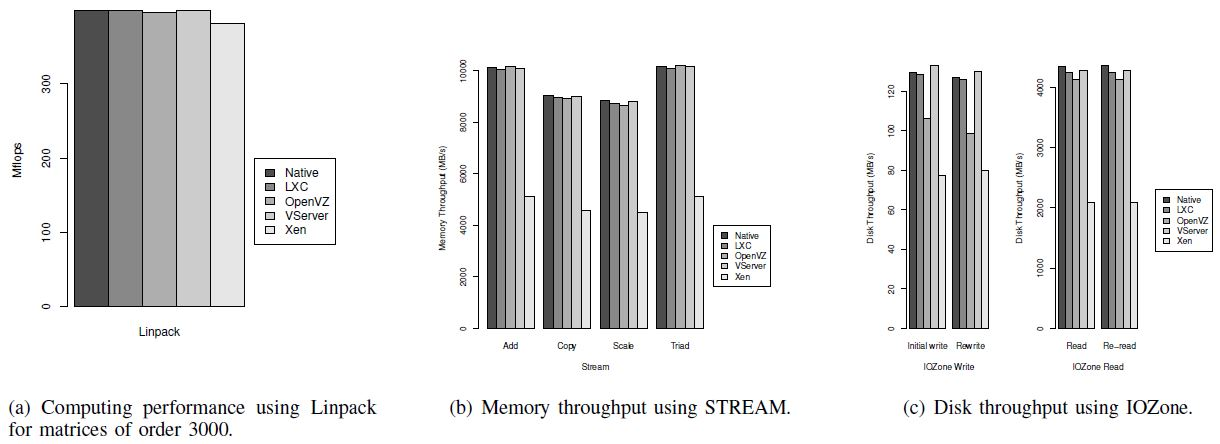
\includegraphics[scale=0.5]{img/performanceBenchmarks.JPG}\\
  \footnotesize\sffamily\textbf{Quelle:} \cite{miguel_g._xavier_performance_????}
  \caption{Performancevergleich von Container- und Hypervisorbasierter Virtualisierung}
  \label{fig:performance_container_hyper}
\end{figure}
In allen gemessenen Feldern bewegte sich die Performance von Containern immer im Bereich der nativen Ausführung und zeigte einen deutlichen Performancevorteil gegenüber der hypervisorbasierten Virtualisierung. 
Ein weiterer Vorteil von Docker gegenüber den klassischen virtuellen Machienen ist die Zeit die benötigt wird um den geforderten Service bereitzustellen. Das Starten einer virtuellen Maschine erfordert auch immer den Start eines Gastbetriebssystems bzw. das Laden eines virtuellen Speicherabbilds. Das starten von Containern hingegen ist nahezu ohne Zeitverlust möglich, da die Anwendung nicht auf deinem Gastbetriebssystem angewiesen ist.
Das Ausführen von Testfällen wird dadurch extrem beschleunigt.


Den Nachteil den Docker allerdings gegenüber echten virtuellen Maschinen hat ist, dass eine Verwendung nur dann Sinn macht, wenn man seine einzelnen Infrastrukturkomponenten auf Linux aufsetzen kann. Da Docker auf den Linux eigenen LXC-Containern aufsetzt können damit auch nur Linux Infrastrukturen emuliert werden.
